%%%%%%%%%%%%%%%%%%%%%%%%%%%%%%%%%%%%%%%%%
% baposter Landscape Poster
% LaTeX Template
% Version 1.0 (11/06/13)
%
% baposter Class Created by:
% Brian Amberg (baposter@brian-amberg.de)
%
% This template has been downloaded from:
% http://www.LaTeXTemplates.com
%
% License:
% CC BY-NC-SA 3.0 (http://creativecommons.org/licenses/by-nc-sa/3.0/)
%
%%%%%%%%%%%%%%%%%%%%%%%%%%%%%%%%%%%%%%%%%

%----------------------------------------------------------------------------------------
%	PACKAGES AND OTHER DOCUMENT CONFIGURATIONS
%----------------------------------------------------------------------------------------

\documentclass[landscape,a0paper,fontscale=0.285]{baposter} % Adjust the font scale/size here

\usepackage{graphicx} % Required for including images
\graphicspath{{../media/}} % Directory in which figures are stored
\usepackage{algorithm, algorithmic}
\usepackage{ mathrsfs }
\usepackage{ dsfont }
\usepackage{amsmath} % For typesetting math
\usepackage{amssymb} % Adds new symbols to be used in math mode

\usepackage{booktabs} % Top and bottom rules for tables
\usepackage{enumitem} % Used to reduce itemize/enumerate spacing
\usepackage{palatino} % Use the Palatino font
\usepackage[font=small,labelfont=bf]{caption} % Required for specifying captions to tables and figures

\usepackage{amsthm}
%\usepackage{amsmath}
\usepackage[english]{babel}
 \theoremstyle{definition}
  \newtheorem{defn}{\protect\definitionname}
   \providecommand{\definitionname}{Definition}


\usepackage{multicol} % Required for multiple columns
\setlength{\columnsep}{1.5em} % Slightly increase the space between columns
\setlength{\columnseprule}{0mm} % No horizontal rule between columns

\usepackage{tikz} % Required for flow chart
\usetikzlibrary{shapes,arrows} % Tikz libraries required for the flow chart in the template

\newcommand{\compresslist}{ % Define a command to reduce spacing within itemize/enumerate environments, this is used right after \begin{itemize} or \begin{enumerate}
\setlength{\itemsep}{1pt}
\setlength{\parskip}{0pt}
\setlength{\parsep}{0pt}
}

\definecolor{lightblue}{rgb}{0.3,0.6,0.9} % Defines the color used for content box headers
\definecolor{darkblue}{rgb}{0.1,0.2,0.3}


%-------------------------------------------------------------------------------
%-------------------------------------------------------------------------------
% Ian's definitions
%-------------------------------------------------------------------------------
%-------------------------------------------------------------------------------

\newtheorem{theorem}{Theorem}
\newtheorem{corollary}{Corollary}
\newtheorem{lemma}{Lemma}
\newtheorem{mydef}{Definition}
\newtheorem{prop}{Proposition}
\newtheorem{claim}{Claim}

% Setting up macro shortcuts
\newcommand{\Exp}{\mathds{E}}
\newcommand{\Expk}{\mathds{E}_{k}}
\newcommand{\Prob}{\mathds{P}}
\newcommand{\Real}{\mathds{R}}
\newcommand{\Nat}{\mathbb{N}}
\newcommand{\Ind}{\mathds{1}}

\newcommand{\Xc}{\mathcal{X}}
\newcommand{\Yc}{\mathcal{Y}}
\newcommand{\Zc}{\mathcal{Z}}
\newcommand{\Pc}{\mathcal{P}}
\newcommand{\Qc}{\mathcal{Q}}
\newcommand{\Fc}{\mathcal{F}}
\newcommand{\Gc}{\mathcal{G}}
\newcommand{\Rc}{\mathcal{R}}
\newcommand{\Sc}{\mathcal{S}}
\newcommand{\Ac}{\mathcal{A}}
\newcommand{\Mc}{\mathcal{M}}
\newcommand{\Tc}{\mathcal{T}}
\newcommand{\Ec}{\mathcal{E}}
\newcommand{\Dc}{\mathcal{D}}
\newcommand{\Dep}{ \Delta^H,\Delta^F,\mathcal{F},\epsilon }

\newcommand{\conf}{\mathcal{F}^d_t}

\newcommand{\vect}[1]{\boldsymbol{#1}}
\newcommand{\opt}{M^*}
\newcommand{\sampled}{{M_k}}
\newcommand{\Pstar}{P^{*}(\cdot \mid s_t, a_t)}
\newcommand{\Pk}{P_{k}(\cdot \mid s_t, a_t)}
\newcommand{\Pdiff}{(P_{k}-P^{*})(\cdot \mid s_t, a_t)}
\newcommand{\Rdiff}{(r_k-r^{*})(s_t, a_t)}
\newcommand{\optPol}{\mu^{*}}
\newcommand{\sampledPol}{\mu_{k}}
\newcommand{\bellmanSampled}{\mathcal{T}_{\mu_{k}(\cdot,i)}^{k}}
\newcommand{\bellmanTrue}{\mathcal{T}_{\mu_{k}(\cdot,i)}^{*}}
\newcommand{\bellmanSampledA}{\mathcal{T}_{\mu_{k}(\cdot,1)}^{k}}
\newcommand{\bellmanTrueA}{\mathcal{T}_{\mu_{k}(\cdot,1)}^{*}}
\newcommand{\vSampled}{V_{\mu_k, 1}^{k}}
\newcommand{\vSampledi}{V_{\mu_k, i}^{k}}
\newcommand{\vTrue}{V_{\tau, \mu_k}^{*}}


%-------------------------------------------------------------------------------
%-------------------------------------------------------------------------------
%-------------------------------------------------------------------------------
%-------------------------------------------------------------------------------


\begin{document}

\begin{poster}
{
headerborder=closed, % Adds a border around the header of content boxes
colspacing=1em, % Column spacing
bgColorOne=white, % Background color for the gradient on the left side of the poster
bgColorTwo=white, % Background color for the gradient on the right side of the poster
borderColor=lightblue, % Border color
headerColorOne=darkblue, % Background color for the header in the content boxes (left side)
headerColorTwo=lightblue, % Background color for the header in the content boxes (right side)
headerFontColor=white, % Text color for the header text in the content boxes
boxColorOne=white, % Background color of the content boxes
textborder=roundedleft, % Format of the border around content boxes, can be: none, bars, coils, triangles, rectangle, rounded, roundedsmall, roundedright or faded
eyecatcher=true, % Set to false for ignoring the left logo in the title and move the title left
headerheight=0.1\textheight, % Height of the header
headershape=roundedright, % Specify the rounded corner in the content box headers, can be: rectangle, small-rounded, roundedright, roundedleft or rounded
headerfont=\Large\bf\textsc, % Large, bold and sans serif font in the headers of content boxes
%textfont={\setlength{\parindent}{1.5em}}, % Uncomment for paragraph indentation
linewidth=2pt % Width of the border lines around content boxes
}
%----------------------------------------------------------------------------------------
%	TITLE SECTION
%----------------------------------------------------------------------------------------
%
{
\includegraphics[height=4em]{logo}} % First university/lab logo on the left
{\bf\textsc{Model-based Reinforcement Learning \\ \vspace{1mm} and the Eluder Dimension}\vspace{0.5em}} % Poster title
{\textsc{ Ian Osband and Benjamin Van Roy \hspace{12pt} Stanford University}} % Author names and institution
{
\includegraphics[height=4em]{logo}} % Second university/lab logo on the right

%----------------------------------------------------------------------------------------
%	Abstract
%----------------------------------------------------------------------------------------

\headerbox{Abstract}{name=abstract,column=0,row=0}{
Any algorithm that applies to all MDPs will suffer $\Omega(\sqrt{|\Sc||\Ac|T})$ regret on some MDP.
So what do we do when \textcolor{magenta}{$|\Sc|, |\Ac|$ are extremely large or infinite}?
The curse of dimensionality means our only hope is to exploit some low-dimensional structure.

\vspace{2mm}
We show that if the MDP can be parameterized within some known function class, we obtain regret \textcolor{magenta}{bounds that scale with the dimensionality, rather than cardinality, of the system}.
We characterize this dependence explicitly in terms of the eluder dimension.
We also present a simple and computationally efficient algorithm (PSRL) that satisfies these bounds.
These are the \textcolor{magenta}{first regret bounds for general model-based learning}.
\vspace{0.3em} % When there are two boxes, some whitespace may need to be added if the one on the right has more content
}

%----------------------------------------------------------------------------------------
%   CONTACT INFORMATION
%----------------------------------------------------------------------------------------

\headerbox{Contact Information}{name=contact,column=3,above=bottom}{ % This block is as tall as the references block
\begin{minipage}[b]{0.75\linewidth}
\vspace{-1mm}
\begin{description}\compresslist
\item[Web] www.stanford.edu/$\sim$iosband
\item[Email] iosband@stanford.edu
\end{description}
% \vspace{1mm}
\end{minipage}
\begin{minipage}[b]{0.2\linewidth}
\begin{flushright}
\vspace{-1mm}

\includegraphics[width=0.5\textwidth]{qr_contact}
% \vspace{1mm}
\end{flushright}
\end{minipage}


}

%----------------------------------------------------------------------------------------
%   REFERENCES
%----------------------------------------------------------------------------------------

\headerbox{References}{name=references,aligned=contact,column=2,above=bottom}{
\begin{minipage}[b]{0.75\linewidth}
\vspace{-1mm}
Please see the full paper: \\
http://arxiv.org/abs/1406.1853
\end{minipage}
\begin{minipage}[b]{0.2\linewidth}
\begin{flushright}
\vspace{-1mm}

\includegraphics[width=0.5\textwidth]{qr_eluder}
% \vspace{1mm}
\end{flushright}
\end{minipage}
}



%----------------------------------------------------------------------------------------
%   Formulation
%----------------------------------------------------------------------------------------

\headerbox{Problem formulation}{name=forumulation,column=0,below=abstract,above=bottom}{

Learn to optimize a random finite horizon MDP $M$ in repeated finite episodes of interaction.

\begin{center}
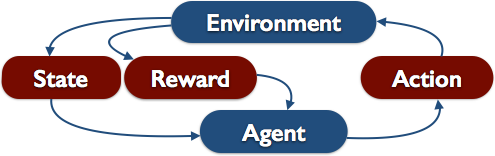
\includegraphics[width=0.8\linewidth]{basic_mdp}
\captionof{figure}{classic reinforcement learning setting}
\end{center}
\vspace{-15pt}

\begin{itemize}\compresslist
\item State space $\Sc$, action space $\Ac$
\item Rewards $r_t \sim R^M(s_t, a_t) \in \Rc$
\item Transitions $s_{t+1} \sim P^M(s_t, a_t) \in \Pc$
\item Epsiode length $\tau$, define $t_k := (k-1) \tau + 1$
\end{itemize}

For MDP $M$ and policy $\mu$, define a value function
\vspace{-3mm}
$$V^{M}_{\mu, i}(s) := \Exp_{M,\mu}\left[ \sum_{j=i}^{\tau} \overline{R}^M(s_j,a_j) \Big| s_i = s \right],$$

\vspace{-1mm} Define the regret in episode $k$ using $\mu_k$ on $M^*$
\vspace{-3mm}
$$\Delta_k := \int_{\Sc} \rho(s) \bigg(\underbrace{V^{M^*}_{\mu^*, 1}(s)}_{\textcolor{magenta}{\text{optimal value}}} - \underbrace{V^{M^{*}}_{\mu_k, 1}(s)}_{\textcolor{magenta}{\text{actual value}}}\bigg)$$

\vspace{-1mm} And finally
${\rm Regret}(T, \pi, M^*) := \sum_{k=1}^{\lceil T/\tau \rceil} \Delta_k$.

\vspace{2mm}
Naive exploration such as Boltzman or $\epsilon$-greedy can lead to exponential regret.
Good performance requires balancing \textcolor{magenta}{\textbf{exploration vs exploitation}}.
}

%----------------------------------------------------------------------------------------
%	Eluder dimension
%----------------------------------------------------------------------------------------

\headerbox{Eluder dimension}{name=eluder,column=1,row=0}{
\begin{center}

\includegraphics[width=0.6\linewidth]{politician.pdf}
\end{center}

\vspace{-3mm}
\textbf{Eluder principle:} a measurement at $x$ is independent of $\{x_1,..,x_n\}$ if functions that are similar at $\{x_1,..,x_n\}$ could differ significantly at $x$.

\vspace{1mm}
\begin{defn}[$ (\mathcal{F},\epsilon)-dependence$]
\hspace{0.00000000000001mm} \newline
We will say that $x \in \mathcal{X}$ is $(\Fc,\epsilon)$-dependent on $\{x_1,...,x_n\} \subseteq \Xc \iff \forall f,\tilde{f} \in \Fc \subseteq \{f: \Xc \rightarrow \Real^n \}$
\vspace{-3mm}
$$\sum_{i=1}^{n} \| f(x_i) - \tilde{f}(x_i) \|_2^2 \le \epsilon^2 \implies \| f(x) - \tilde{f}(x)\|_2 \le \epsilon.$$

\vspace{-3mm}
$x \in \mathcal{X}$ is $(\epsilon,\mathcal{F})$-independent of $\{x_1,..,x_n\}$ iff it does not satisfy the definition for dependence.
\end{defn}

\vspace{-3mm}
\begin{center}
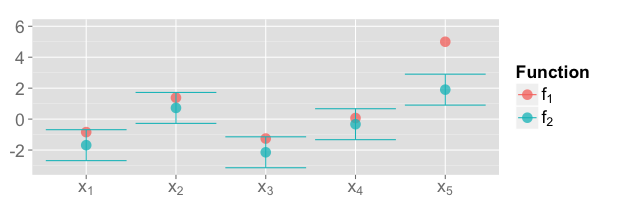
\includegraphics[width=0.85\linewidth]{eps_dependence}
\vspace{-3mm}
\captionof{figure}{$x_5$ is $(\{f_1, f_2\},1)$-independent of $\{x_1, .., x_4\}$.}
\end{center}

\vspace{-7mm}
\textcolor{magenta}{\begin{defn}[Eluder Dimension $= {\rm dim}_E(\Fc,\epsilon)$]
\label{def: Eluder} \hspace{0.00000000000001mm} \newline
\textcolor{black}{The length of the longest possible sequence of elements in $\Xc$ such that for some $\epsilon' \ge \epsilon$ every element is $(\Fc,\epsilon')$-independent of its predecessors.}
\end{defn}
}

\vspace{-1mm}
\textbf{Examples}
\begin{itemize}[noitemsep,nolistsep]
    \item $\Xc$ finite $\implies$ ${\rm dim}_E(\Fc, \epsilon) \le |\Xc|$.
    \item $\Fc \subseteq \{f: \Real^n \rightarrow \Real^p \text{ linear} \}$ \\ $\implies$ ${\rm dim}_E(\Fc, \epsilon) = O\left(np \log(1/\epsilon)\right)$
\end{itemize}

}

%----------------------------------------------------------------------------------------
%   Kolmogorov dimension
%----------------------------------------------------------------------------------------

\headerbox{Kolmogorov dimension}{name=kolmogorov,column=1,span=1,row=0, below=eluder, above=bottom}{
The Kolmogorov dimension of a function class $\Fc$:
\vspace{-4mm}
$$ {\rm dim}_K(\Fc) := \limsup_{\alpha \downarrow 0} \frac{\log(\overbrace{N(\Fc,\alpha,\|\cdot\|_2)}^{\alpha-\text{covering number}})}{\log(1/\alpha)} .$$

\vspace{-3mm}
\begin{minipage}[b]{0.45\linewidth}
\centering
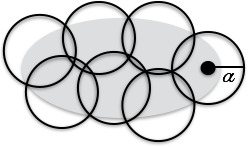
\includegraphics[width=\textwidth]{covering}
\end{minipage}
\vspace{-10mm}
\begin{minipage}[b]{0.5\linewidth}
\centering


In this diagram $N(\Fc,\alpha,\|\cdot\|_2) \le 7$

\vspace{3mm}
\textbf{Example:} ${\rm dim}_K(\Real^d) = d$

\vspace{1mm}
\end{minipage}
}


%----------------------------------------------------------------------------------------
%   Lipschitz constant
%----------------------------------------------------------------------------------------

\headerbox{Lipschitz smoothness}{name=lipschitz,column=2,span=1,row=0}{
\begin{defn}[Future value function $U^M_i$]
\hspace{0.0001mm} \newline
For any distribution $\Phi$ over $\Sc$ we define:
\vspace{-2mm}
$$U^M_{i}(\Phi) := \Exp_{M,\mu^M}\big[ V^M_{\mu^M,i+1}(s) \big| s \sim \Phi \big]$$

\vspace{-2mm}
as the value of the optimal policy, starting from $\Phi$.
\end{defn}


\begin{itemize}[leftmargin=*]
    \item Learning an infinite MDP requires regularity
    \item Assume $U^{M^*}_i$ is Lipschitz in $\Exp[s | s \sim \Phi]$ wrt $\| \cdot \|_2$
    \item Satisfied whenever $V^{M^*}_{\mu^*, i}$ Lipschitz in $s$ wrt $\| \cdot \|_2$
    \item But this is a strictly weaker condition since \\ system noise can help smooth future value.
\end{itemize}

}

%----------------------------------------------------------------------------------------
%   Posterior sampling
%----------------------------------------------------------------------------------------

\headerbox{Posterior Sampling}{name=posterior,column=2,span=1,row=0, below=lipschitz}{
For each episode $k$:
\vspace{-1mm}
\begin{enumerate}\compresslist
\item Sample an MDP from the posterior distribution for the true MDP: $M_k \sim \phi(\cdot | H_t)$.
\vspace{1mm}
\item Use policy $\mu_k \in \underset{\mu}{\arg\max} V^{M_k}_\mu$.
\end{enumerate}
\vspace{-2mm}
}


%----------------------------------------------------------------------------------------
%   Main Results
%----------------------------------------------------------------------------------------

\headerbox{Main results}{name=main,column=2,below=posterior, above=references}{
If $M^*$ is an MDP with rewards $R^* \in \Rc $ and transitions $P^* \in \Pc $ with sub $\sigma$-Gaussian noise then the \textcolor{magenta}{expected regret} to time $T$ of PSRL is bounded:

\vspace{-2mm}
{\small
\textcolor{magenta}{
$$\tilde{O} \bigg( \underbrace{\sigma_\Rc \\ \sqrt{d_K(\Rc) d_E(\Rc) T}}_{\text{rewards}} + \underbrace{\Exp[K^*]}_{\text{Lipschitz}} \underbrace{\sigma_\Pc \sqrt{d_K(\Pc) d_E(\Pc) T}}_{\text{transitions}} \bigg) $$}
}

\vspace{-3mm}
\textbf{Notation:}
\begin{itemize}[leftmargin=*,noitemsep,nolistsep]
    \item {Kolmogorov dimension $d_K(\Fc)$} $:= {\rm dim}_K(\Fc)$
    \item {Eluder dimension $d_E(\Fc)$} $:= {\rm dim}_E(\Fc, T^{-1})$
    \item {Lipschitz constant $K^*$} for future value function
\end{itemize}

\vspace{2mm}
\textbf{Corollary:}\\
Let $M^*$ be a linear-quadratic system in $\Real^d$ with $\sigma$-sub-Gaussian noise mean-bounded by $C$ then:
\vspace{-3mm}
$$\Exp[{\rm Regret}(T,\pi^{PS},M^*)] = \underbrace{\tilde{O} \left( \sigma C d^2 \sqrt{T} \ \right)}_{\textcolor{magenta}{\text{no exponential scaling in }d}}.$$
}




%----------------------------------------------------------------------------------------
%   Optimism
%----------------------------------------------------------------------------------------

\headerbox{Proof sketch}{name=proof,column=3,span=1,row=0}{
We consider the regret in an episode $k$:
\vspace{-1mm}
\begin{eqnarray*}
    \Delta_k &=&  V^*_{*,1}(s) - V^*_{k,1}(s)\\
     &=& \underbrace{\big( V^k_{k,1}(s) - V^*_{k,1}(s) \big)}_{\text{Imagined - Actual}}
     + \underbrace{\big(V^*_{*,1}(s) - V^k_{k,1}(s) \big)}_{\Exp[\cdot] = 0 \text{ by posterior}}
\end{eqnarray*}

\vspace{-1mm}
We can decompose this into Bellman error:
\vspace{-3mm}
\begin{equation*}
    V^k_{k,1} - V^*_{k,1} =
    \underbrace{\sum_{i=1}^\tau \left( \Tc^k_{k,i} - \Tc^*_{k,i} \right) V^k_{k,i+1}}_{\textcolor{magenta}{B := \text{Bellman error}}}
    + \underbrace{ \sum_{i=1}^\tau d_{t_k+1}}_{\Exp=0 \text{ martingale}}.
\end{equation*}

\vspace{-1mm}
We can now use the H\"{o}lder inequality to bound:
\vspace{-3mm}
\begin{equation*}
\label{eq: err sums}
    \textcolor{magenta}{B} \le \sum_{i=1}^\tau \bigg\{
    \underbrace{|\overline{R}^k - \overline{R}^* |}_{\text{reward error}}
    + \underbrace{K^k}_{\text{Lipschitz}} \underbrace{\|P^k - P^* \|_2}_{\text{transition error}}
    \bigg\}
\end{equation*}

\vspace{-1mm}
We conclude the proof by upper bounding these deviations in terms of our estimation errors on $R^*$ and $P^*$.
We use concentration inequalities to express the error bounds for $\Rc$ and $\Pc$ in terms of the eluder dimension and Kolmogorov dimension.

\vspace{2mm}
\textbf{Note} a proof for a similar optimistic algorithm is possible, however this would require a generally intractable planning step.
We believe that the sampling approach will also be more statistically efficient since it is not affected by loose analysis.
}


%----------------------------------------------------------------------------------------
%   ANALYSIS
%----------------------------------------------------------------------------------------



\headerbox{So what?}{name=example,column=3,span=1,row=0, below=proof, above=references, borderColor=magenta, headerColorTwo=magenta}{
\bf
\begin{itemize}[leftmargin=*]
    \item Practical reinforcement learning problems \\ often have $|\Sc|$ and $|\Ac|$ very large or infinite.
    \item ``Tabula rasa'' learning will always require minimum $T=\Omega(|\Sc||\Ac|)$ for good guarantees $\implies$ must exploit low-dimensional structure.
    \item \textcolor{magenta}{We produce a unified analysis for model-based RL in terms of the dimensionality, rather than the cardinality, of the system}.
    \item Conceptually simple, computationally efficient algorithm PSRL satisfies these bounds.
\end{itemize}
}





%----------------------------------------------------------------------------------------

\end{poster}

\end{document}
